\Chapter{Az oldalnézetes játékok, valamint a játékmotorok jellemzői}

\Section{A fejezet célja}

Ebben a fejezetben arra fogok törekedni, hogy részletesen bemutassam az oldalnézetes (side-scroller) játékok és a pályageneráló algoritmusok világát. Megvizsgálom az oldalnézetes játékok történelmi fejlődését, általános jellemzőit, és azt, hogy hogyan kapcsolódnak ezek a játéktípusok a pályageneráláshoz.

Ezen felül részletezni fogom a játékmotorok különböző típusait, előnyeit és hátrányait.

A hivatkozások jelentős része ehhez a fejezethez szokott kötődni.
(Egy hivatkozás például így néz ki \cite{redbull}.)
Itt lehet bemutatni a hasonló alkalmazásokat.

\Section{Az oldalnézetes játékok}

\SubSection{Fejlődésük}
A 2D-s platformjátékok fejlődése gazdag és változatos utazás a videójátékok történetében. Egy rövid áttekintést szeretnék adni a fejlődésükről:
\begin{enumerate}
\item A kezdetek: Ez a műfaj a „Space Panic”-kel (1980) kezdődött, de a „Donkey Kong” (1981) volt az, amely a létrák és az ugrálás kombinálásával igazán megteremtette a mércét. Ezek a korai játékok többnyire egyképernyős platformerek voltak.\cite{redbull}
\item „Side-scroller” korszak: A „Super Mario Bros.” (1985) forradalmasította a műfajt a „side-scroller” pályákkal, emlékezetes karaktereket, „power-up”-okat és titkos útvonalakat vezetve be. Ebben a korszakban olyan játékok is megjelentek, mint a „Mega Man” és a „Metroid”, amelyek ezt a típusú játékstílust más elemekkel, például lövöldözéssel és felfedezéssel vegyítették.\cite{redbull} A Super Mario Bros. játékmenete \aref{fig:supermariobros}. ábrán látható.
\begin{figure}[ht]
\centering
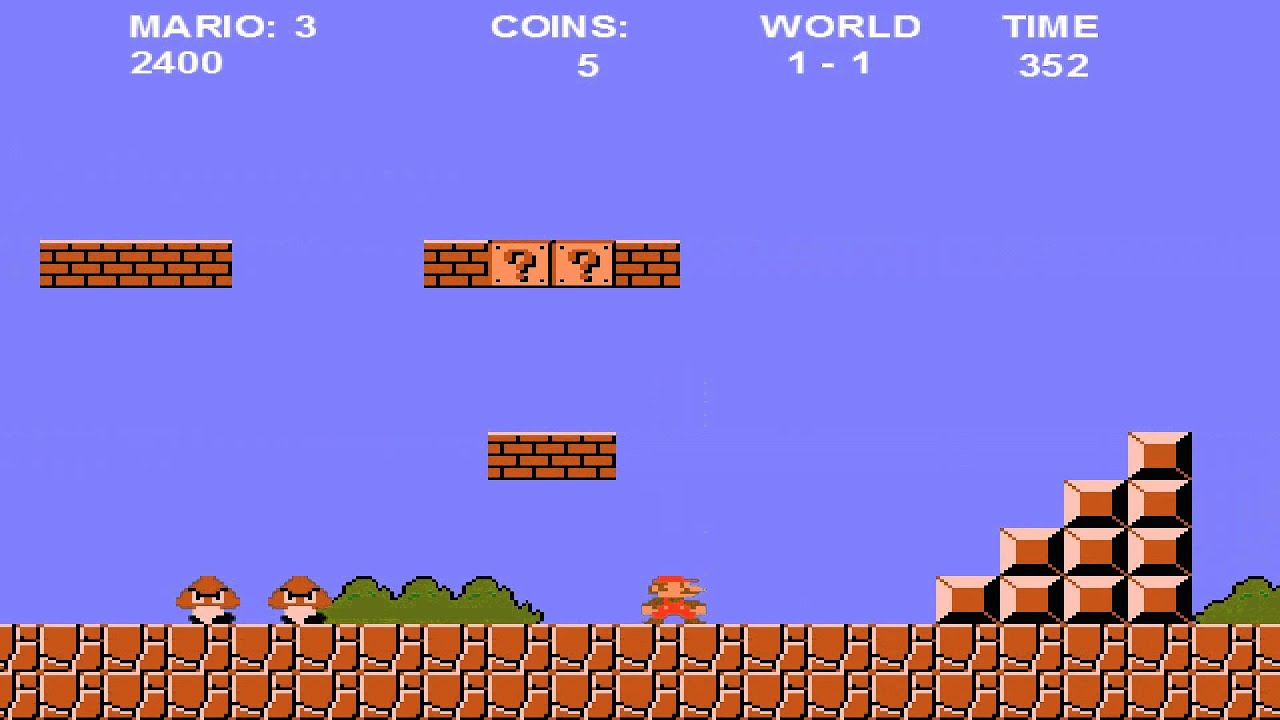
\includegraphics[scale=0.3]{images/super_mario_bros.jpg}
\caption{A Super Mario Bros. játékmenete}
\label{fig:supermariobros}
\end{figure}
\item A technológia fejlődése: A technológia fejlődésével a játékok elkezdtek pszeudo-3D elemeket tartalmazni. Az 1990-es években az olyan játékok, mint a „Crash Bandicoot” a platformer koncepciókat valódi 3D-s környezetbe helyezték.\cite{redbull}
\item A 16 bites korszak: A „Mega Man X” és a „Donkey Kong Country” figyelemre méltó példái ennek az időszaknak. A 16 bites konzolok bevezetése lehetővé tette a feljavított párhuzamos görgetést és a részletesebb sprite-okat.\cite{redbull}
\item  Korai 3D korszak: A korai 3D platformerek közé tartoztak a 2,5D-s címek és a 3D-s perspektívájú, de 2D-s grafikájú platformerek. Az olyan játékok, mint a "Crash Bandicoot", lineáris pályákon maradtak, de vegyítették a járműveket és a másodpercek töredékeiben történő platformozást.\cite{redbull} A Crash Bandicoot játék \aref{fig:crashbandicoot}. ábrán látható.
\begin{figure}[ht]
\centering
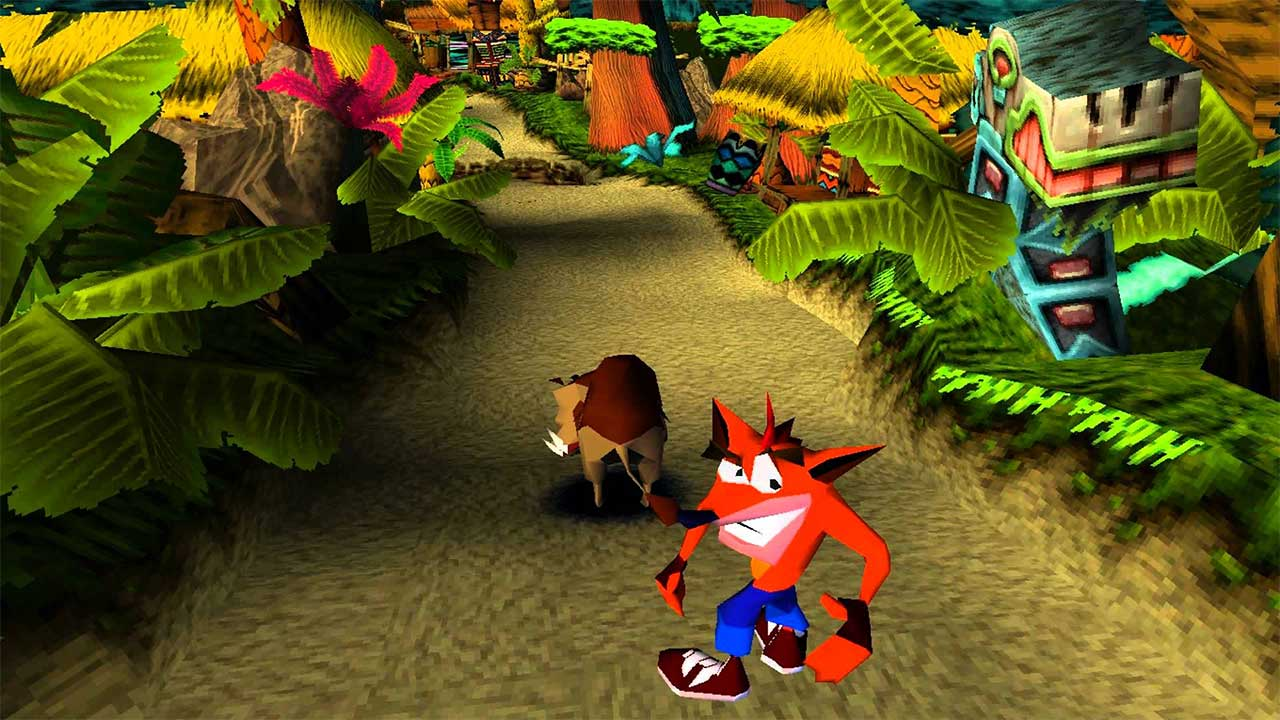
\includegraphics[scale = 0.3]{images/crashbandicoot.png}
\caption{A Crash Bandicoot játék}
\label{fig:crashbandicoot}
\end{figure}
\item Az indie újjáéledés: A 2000-es évek végén és a 2010-es években az indie fejlesztők jelentős szerepet játszottak a 2D-s platformjátékok újjáélesztésében, és inkább a történetre és az innovációra összpontosítottak. Az olyan játékok, mint a "Braid", a "Limbo" és a "Super Meat Boy" egyedi mechanikájukkal és narratívájukkal mutatták be ezt a trendet.\cite{redbull} A Limbo játék \aref{fig:limbo}. ábrán megtekinthető.
\begin{figure}[ht]
\centering
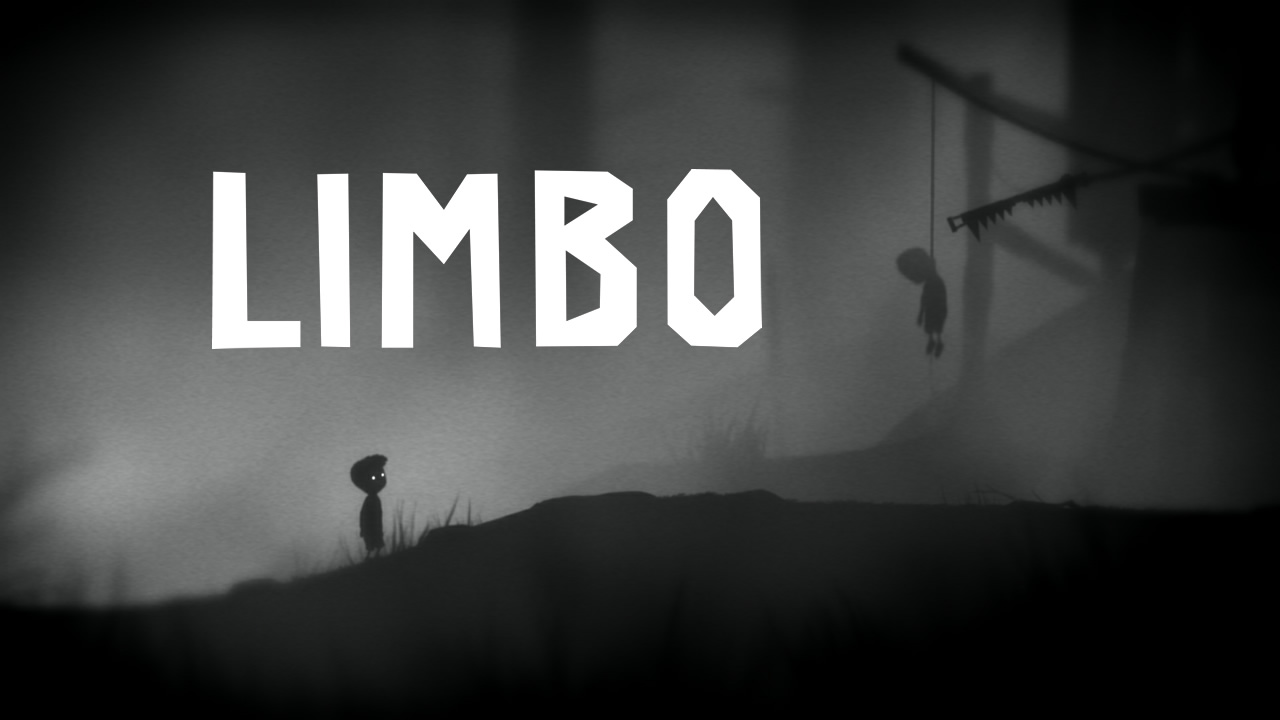
\includegraphics[scale = 0.3]{images/limbo.jpg}
\caption{A Limbo játék}
\label{fig:limbo}
\end{figure}
\item Modern korszak: A 2D platformjátékok az utóbbi években továbbra is népszerűek, gyakran a hagyományos játékmenetet modern tervezési elvekkel ötvözik. Az olyan címek, mint a "New Super Mario Bros." sorozat és a különböző indie játékok élénk és változatos műfajt tartanak fenn.\cite{redbull}
\end{enumerate}

\SubSection{Általános jellemzőik}

A platformer játék, más néven platform videojáték, egy olyan játéktípus, amely jellemzően kétdimenziós grafikával rendelkezik, és amelyben a játékosok a képernyőn különböző platformokon ugráló vagy mászkáló karaktereket irányítanak.

A platformjátékokban egy karakter egy pályán navigál, hogy feladatokat teljesítsen, magas pontszámokat érjen el, vagy egyszerűen csak életben maradjon. Mivel ez a játékműfaj az évek során jelentősen megváltozott, sok ilyen játéknak más lehet a látványvilága. A következő jellemzők azonban gyakran megtalálhatók a platformjátékokban.\cite{platformerfeature}
\begin{itemize}
\item Interaktív környezet: Azt, hogy egy karakter mit tehet egy játékban, nagyban befolyásolja a szint vagy a környezet kialakítása. A platformjátékok célja különösen az, hogy próbára tegyék a játékost, miközben a főhőst olyan összetett akadályok elé állítja, mint a szöges platformok, halálos csapdák vagy lávával esetleg vízzel teli szakadékok.\cite{platformerfeature}
\item Third-Person nézőpont: A játékos által irányított karakter az előtte lévő képernyőn látható, mivel sok platformjátékot úgynevezett „third-person” perspektívából készítenek.\cite{platformerfeature}
\item Vízszintes és függőleges mozgás: A platformjátékok többsége kétdimenziós „side-scroller” játék, ami azt jelenti, hogy a játékos oldalról látja a karakterét, miközben a képernyő vízszintesen vagy függőlegesen mozog vele együtt.\cite{platformerfeature} A horizontális és vertikális mozgásról egy kép \aref{fig:horvermovement}. ábrán látható.
\begin{figure}[ht]
\centering
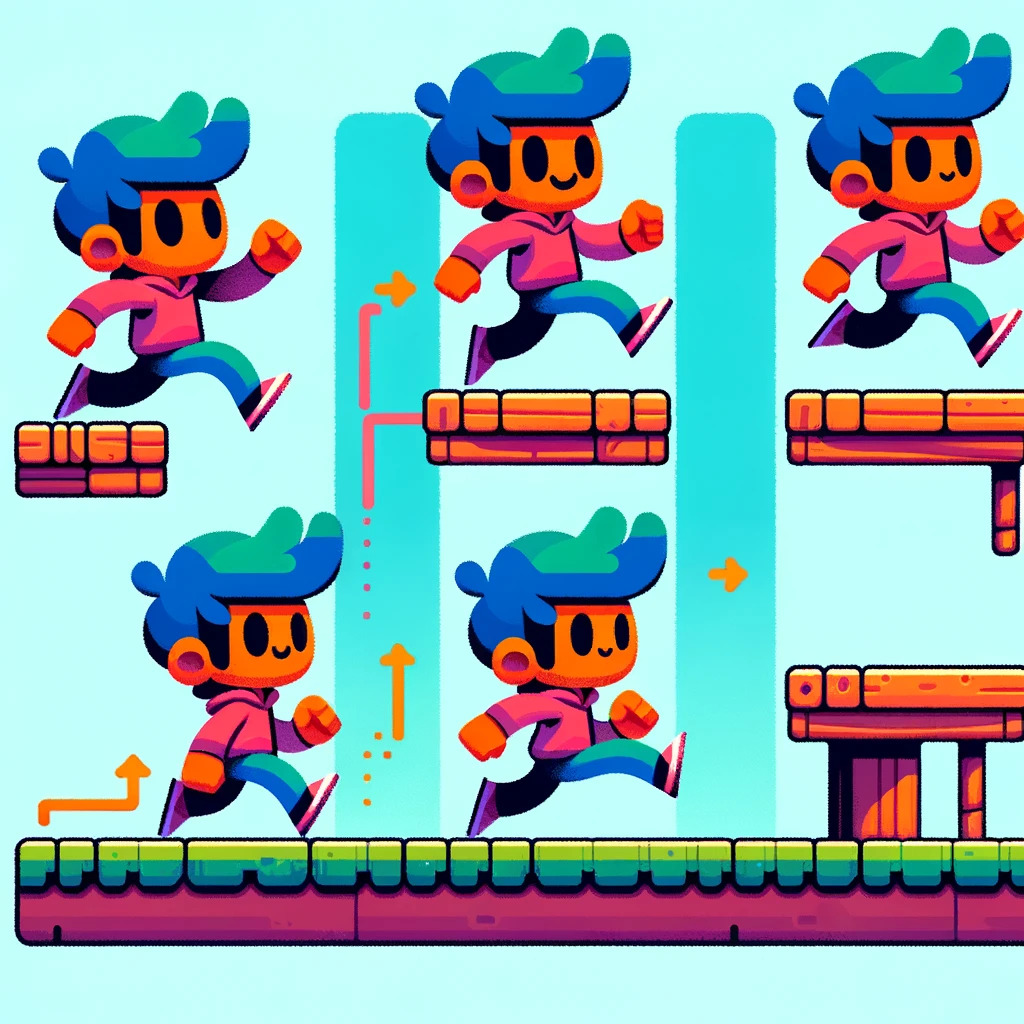
\includegraphics[scale = 0.3]{images/vertical_and_horizontal_movement.jpg}
\caption{A horizontális és vertikális mozgás}
\label{fig:horvermovement}
\end{figure}
\item Az ugrás kontrollálása: A játékos irányítja a karakter ugrási képességét, ami a platformjátékok egyik fő szempontja. Ezekben a játékokban az ugrás gyakran szükséges a környezetben való mozgáshoz és a következő szintre jutáshoz.\cite{platformerfeature}
\item Történetmesélés és világépítés: Bár a korai platformjátékokban nem volt ennyire elterjedt, a modern 2D-s platformjátékok gyakran tartalmaznak gazdag történetmesélést és részletes világépítést a játékélmény fokozása érdekében.\cite{platformerfeature}
\end{itemize}
Ezek a funkciók együttesen hozzák létre azt az egyedi és gyakran kihívást jelentő élményt, amely a 2D platformer játékokat jellemzi. A műfaj az évek során jelentősen fejlődött, és minden játék a maga újításait és fordulatait vezette be ezekbe az alapvető összetevőkbe.

\SubSection{A pályageneráló algoritmusok kapcsolódása a platformer játékokhoz}

A számítógépes játékokban sokszor sokkal több tartalom megjelenítését szeretnénk elérni, mint amennyit valójában elő tudunk állítani vagy el tudunk tárolni. Vagy a tartalom előállítása során felmerülő korlátozások miatt - pl. egy kis gyártócsapat esetében -, vagy a tartalom tárolása, esetleg forgalmazása miatt. \cite{platformerconnection}

Ezt azonban megkerülhetjük a procedurális generálással. Ez az, amikor a játék menetközben, játékidőben generál új tartalmat, ahelyett, hogy csak a korábban előállított tartalmat használná fel. Ha jól csináljuk, ez gyakorlatilag korlátlan tartalmat biztosíthat a játékunkban, sokkal alacsonyabb előzetes előállítási költségekkel.\cite{platformerconnection}

A 2D-s platformjátékokban a térképgeneráló algoritmusok döntő szerepet játszanak a dinamikus és magával ragadó játékkörnyezetek létrehozásában. Ezek az algoritmusok generálhatnak térképeket előre létező szakaszok összerakásával vagy változó terepviszonyokkal rendelkező tájak rajzolásával. Egy gyakori módszer egy alapvonal megrajzolása (amely a talajt jelképezi), majd annak a magasságának a tájban való megváltoztatása a változatosság megteremtése érdekében.\cite{platformerconnection}

Ezeknek az algoritmusoknak a 2D platformerekben való használata lehetővé teszi egyedi, procedurálisan generált világok létrehozását, ami növeli az újrajátszhatóságot és a játékosok érdeklődését. Minden egyes játékmenet más-más élményt nyújthat, a tájak az egyszerű és lapostól a komplex és többszintesig terjedhetnek.\cite{platformerconnection}

Több játék is nagyszerűen használta az procedurális generálást. Például a Roguelight című játék,amely \aref{fig:rougelight}. ábrán látható, bemutatja, hogy a procedurális generálással hogyan lehet mélyebb és sötétebb környezetet létrehozni, amely minden egyes játékmenettel változik.

\begin{figure}[ht]
\centering
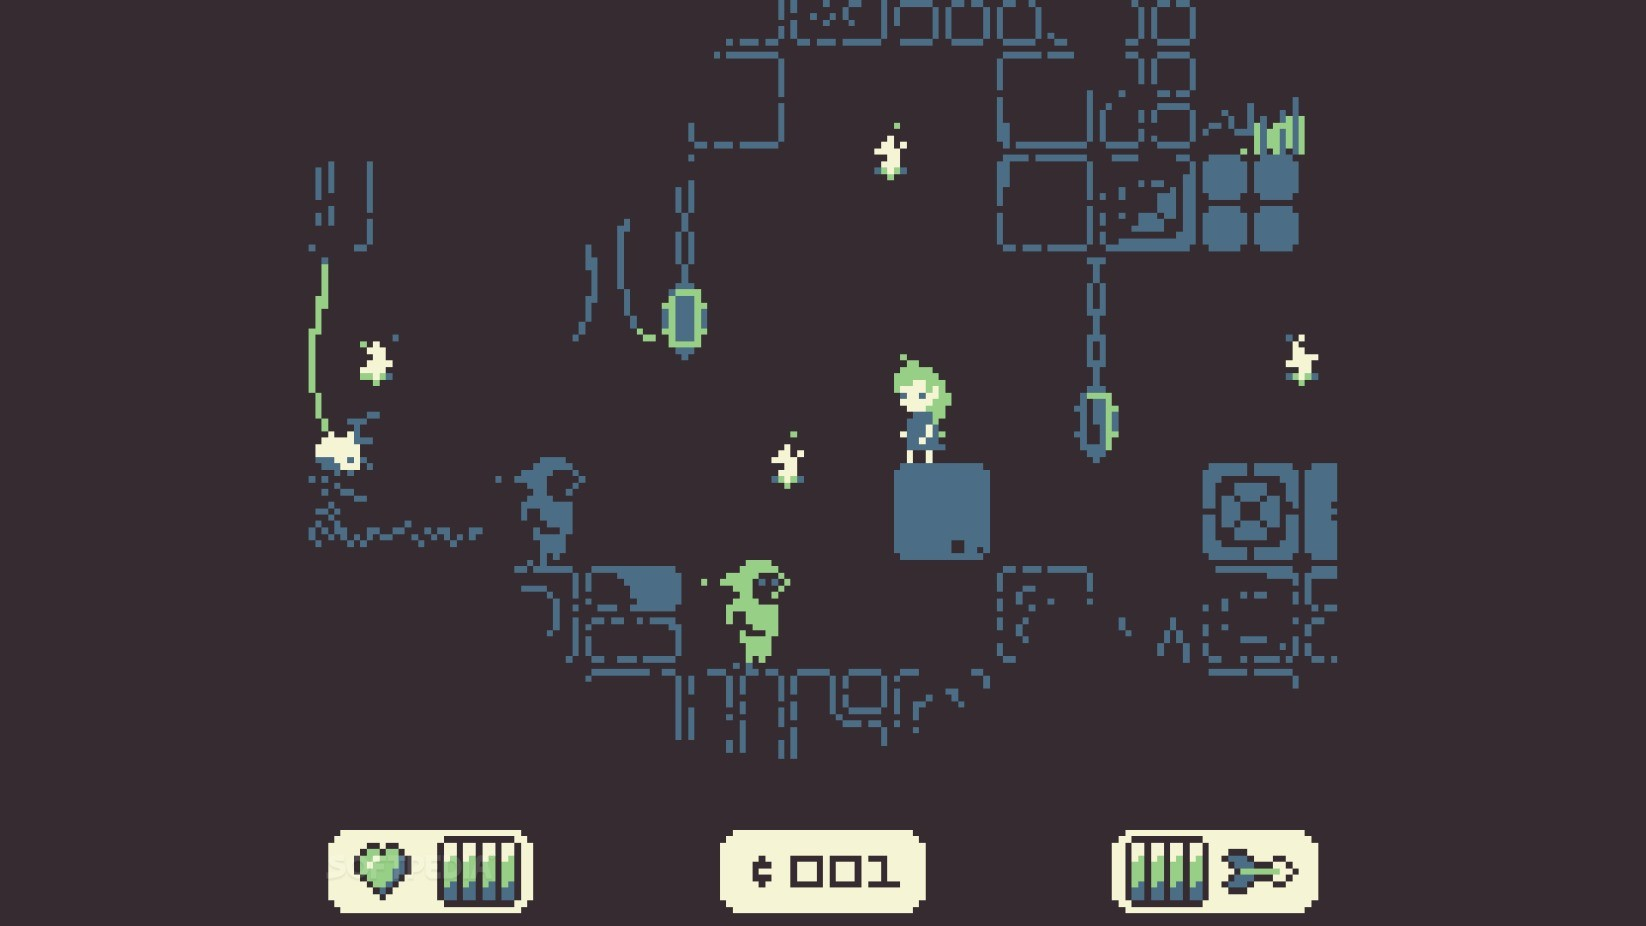
\includegraphics[scale = 0.2]{images/rougelight.jpg}
\caption{A Rougelight játék}
\label{fig:rougelight}
\end{figure}

A "Diskophoros" egy másik érdekes cím, amely a gyors tempójú multiplayer akciót procedurálisan generált pályákkal kombinálja, így minden egyes játékmenet során új élményt tud nyújtani a játékosok számára. A Diskophoros játék \aref{fig:diskophoros}. ábrán látható.

\begin{figure}[ht]
\centering
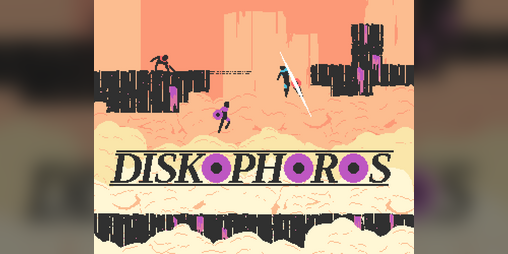
\includegraphics[scale = 0.7]{images/diskophoros.png}
\caption{A Diskophoros játék}
\label{fig:diskophoros}
\end{figure}

Ezek a példák szemléltetik a procedurális térképgenerálás változatos alkalmazásait a 2D-s platformjátékokban, jelentősen hozzájárulva a játéktervezéshez és a játékosok általi érdeklődés növeléséhez.

\newpage

\Section{Játékmotorok}

A játékmotor olyan szoftveres keretrendszer, amelyet elsősorban videojátékok fejlesztésére terveztek. Ezek a motorok lehetővé teszik a játékfejlesztő cégek számára, hogy az összes munkájukat egy kész termékké egyesítsék. Manapság majdnem minden videójáték egy játékmotor segítségével készült. Azért nevezzük „motoroknak”, mivel ezek működtetik a teljes játékvilágot, amit az ember elé tárnak.\cite{gameengine1}

A játékmotorok igen sokféle funkciót kínálnak, például 2D vagy 3D grafikus megjelenítést, ütközésérzékelő és -reagáló fizikamotort, hangot, szkriptelést, animációt, mesterséges intelligenciát, hálózatot, streaminget, memóriakezelést, szálkezelést, lokalizációs támogatást, jelenetgrafikát és videótámogatást a filmes jelenetekhez. Ezek a funkciók megkönnyítik a játékfejlesztés összetett folyamatait azáltal, hogy automatizálják a legtöbb játékprojektben előforduló ismétlődő feladatokat és így jelentősen csökkentik a költségeket, a komplexitást és a piacra kerülési időt.\cite{gameengine1}

A játékmotoroknak két fő típusa van: a harmadik féltől származó motorok és a saját fejlesztésű motorok. A harmadik féltől származó motorokat vállalatok fejlesztik ki, hogy más stúdióknak adják bérbe őket. Ezeket a motorokat úgy tervezték, hogy különböző játékműfajokat és játékstílusokat támogassanak. A jól ismert harmadik féltől származó motorok közé tartozik az Unreal Engine és a Unity. Ugyanakkor a saját fejlesztésű motorokat egy játékstúdió házon belül, konkrét projektekhez fejleszti, ami lehetővé teszi a játék követelményeihez jobban illeszkedő és testre szabható funkciókat.\cite{gameengine1}

A játékmotorokat a játékfejlesztő csapat szinte minden tagja használja. A pályatervezők, az animátorok és a környezettervező művészek jelentős időt töltenek a motoron belüli munkával, a játék különböző elemeit alakítva a környezettől kezdve a karakterek mozgatásán át a világításig.\cite{gameengine1}

A megfelelő játékmotor megválasztása több tényezőtől függ, például a projekt-költségvetéstől, a játék terjedelmétől, valamint a játékfejlesztő cég méretétől is függhet. Míg a kisebb stúdiók a költség- és erőforrás-korlátok miatt harmadik féltől származó motorok mellett dönthetnek, addig a nagyobb, több erőforrással rendelkező stúdiók saját motorokat fejleszthetnek a játékuk speciális igényeinek kielégítésére.\cite{gameengine1}

\SubSection{Az Unreal Engine játékmotor}

Az Epic Games által fejlesztett Unreal Engine gazdag múltra tekint vissza a videojáték-fejlesztés világában. A motort eredetileg Tim Sweeney alkotta meg az 1998-ban megjelent "Unreal" című „first-person” lövöldözős játékhoz, de az évek során jelentősen fejlődött. Az első generációja a szoftveres renderelési képességeiről volt nevezetes, később pedig a dedikált grafikus kártyák teljesítményének kihasználásáról.\cite{unrealengine1}

Az Unreal Engine egy teljes körű, fejlett fizikai motorral rendelkező, nyílt forráskódú játékmotor, amelyet, ha nem kereskedelmi célra használunk, akkor ingyenes. Az Unreal Engine emellett támogatja a különböző platformokra való telepítést, többek között a Windows PC, PlayStation, Xbox, macOS, iOS és Android platformokra, és visszafelé kompatibilis az Unreal Engine 4 egyes korábbi verzióival. A játékmotort C++ nyelven írták, és ez is a hivatalos scripting nyelve, de a kezdő programozók bátran használhatják a motor Blueprint névre hallgató visual scripting rendszerét, amely \aref{fig:unrealblueprint}. ábrán látható.\cite{unrealengine1}

\begin{figure}[ht]
\centering
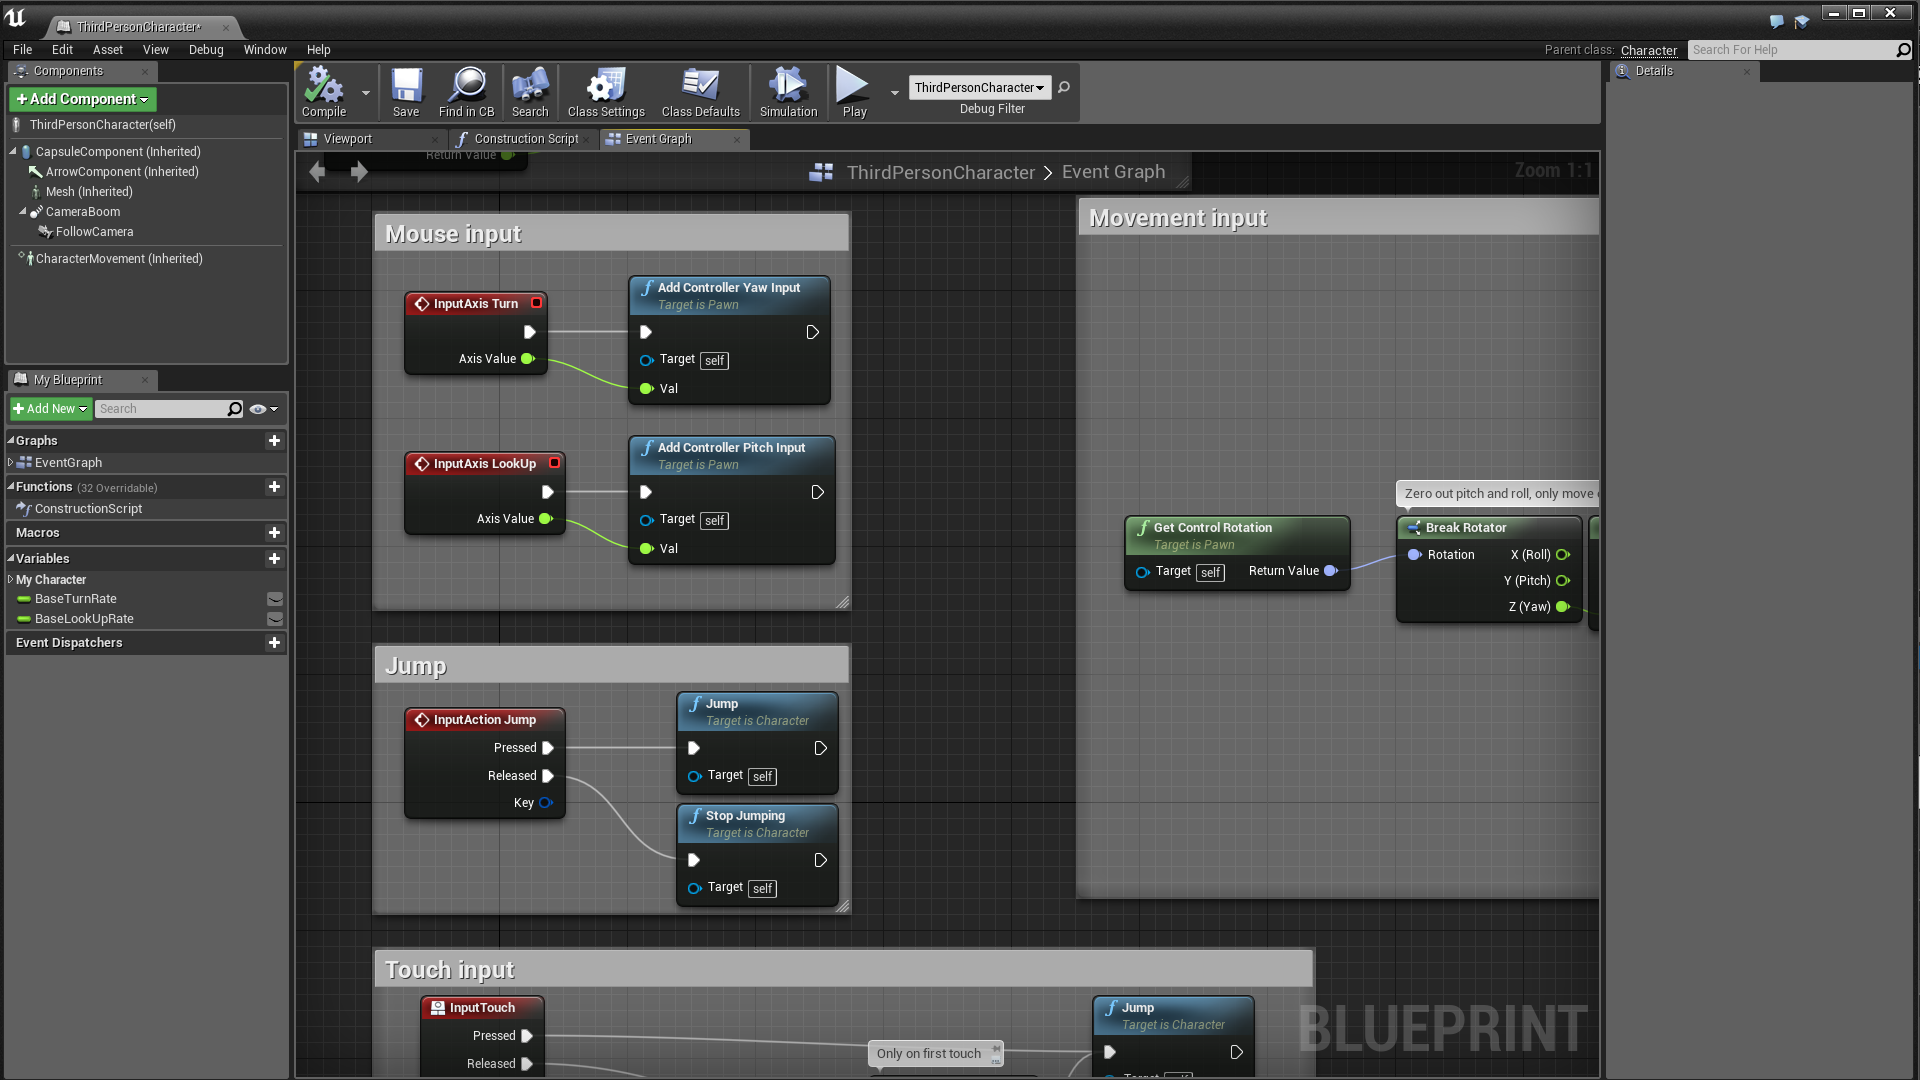
\includegraphics[scale = 0.2]{images/blueprinteditor_windows.png}
\caption{Az Unreal Engine Blueprint nevezetű visual scripting rendszere\cite{unrealengine2}}
\label{fig:unrealblueprint}
\end{figure}

Az Unreal Engine népszerűsége és sokoldalúsága nem csak a rendkívül valósághű grafikai képességeinek köszönhető, hanem annak is, hogy a játékokon kívül is széles körben használják, például a film- és televíziós produkciókban.

\SubSection{A Godot játékmotor}

A Godot Engine egy sokoldalú, ingyenes és nyílt forráskódú játékmotor 2D-s és 3D-s játékok készítéséhez. A Godot lehetővé teszi a videojáték-fejlesztők számára, hogy 3D-s és 2D-s játékokat készítsenek több programozási nyelv, például C++, C\# és GDScript használatával. A programozásban kevésbé jártas játékfejlesztők használhatják a Godot visual scripting funkcióját is, amely \aref{fig:godotengine}. ábrán látható. A fejlesztés megkönnyítése érdekében csomópontok hierarchiáját használja. Egy csomóponttípusból osztályok származtathatók, hogy speciálisabb csomóponttípusokat hozzanak létre, amelyek öröklik a viselkedést. A Godot szerkesztője támogatja az olyan asztali platformokat, mint a Linux, a macOS és a Windows, valamint az androidos telefonokat és táblagépeket. Bár konzolokon is futtatható, a nyílt forráskódú licenckorlátozások miatt a népszerű konzolok hivatalos támogatása nem érhető el.\cite{godot}

\begin{figure}[ht]
\centering
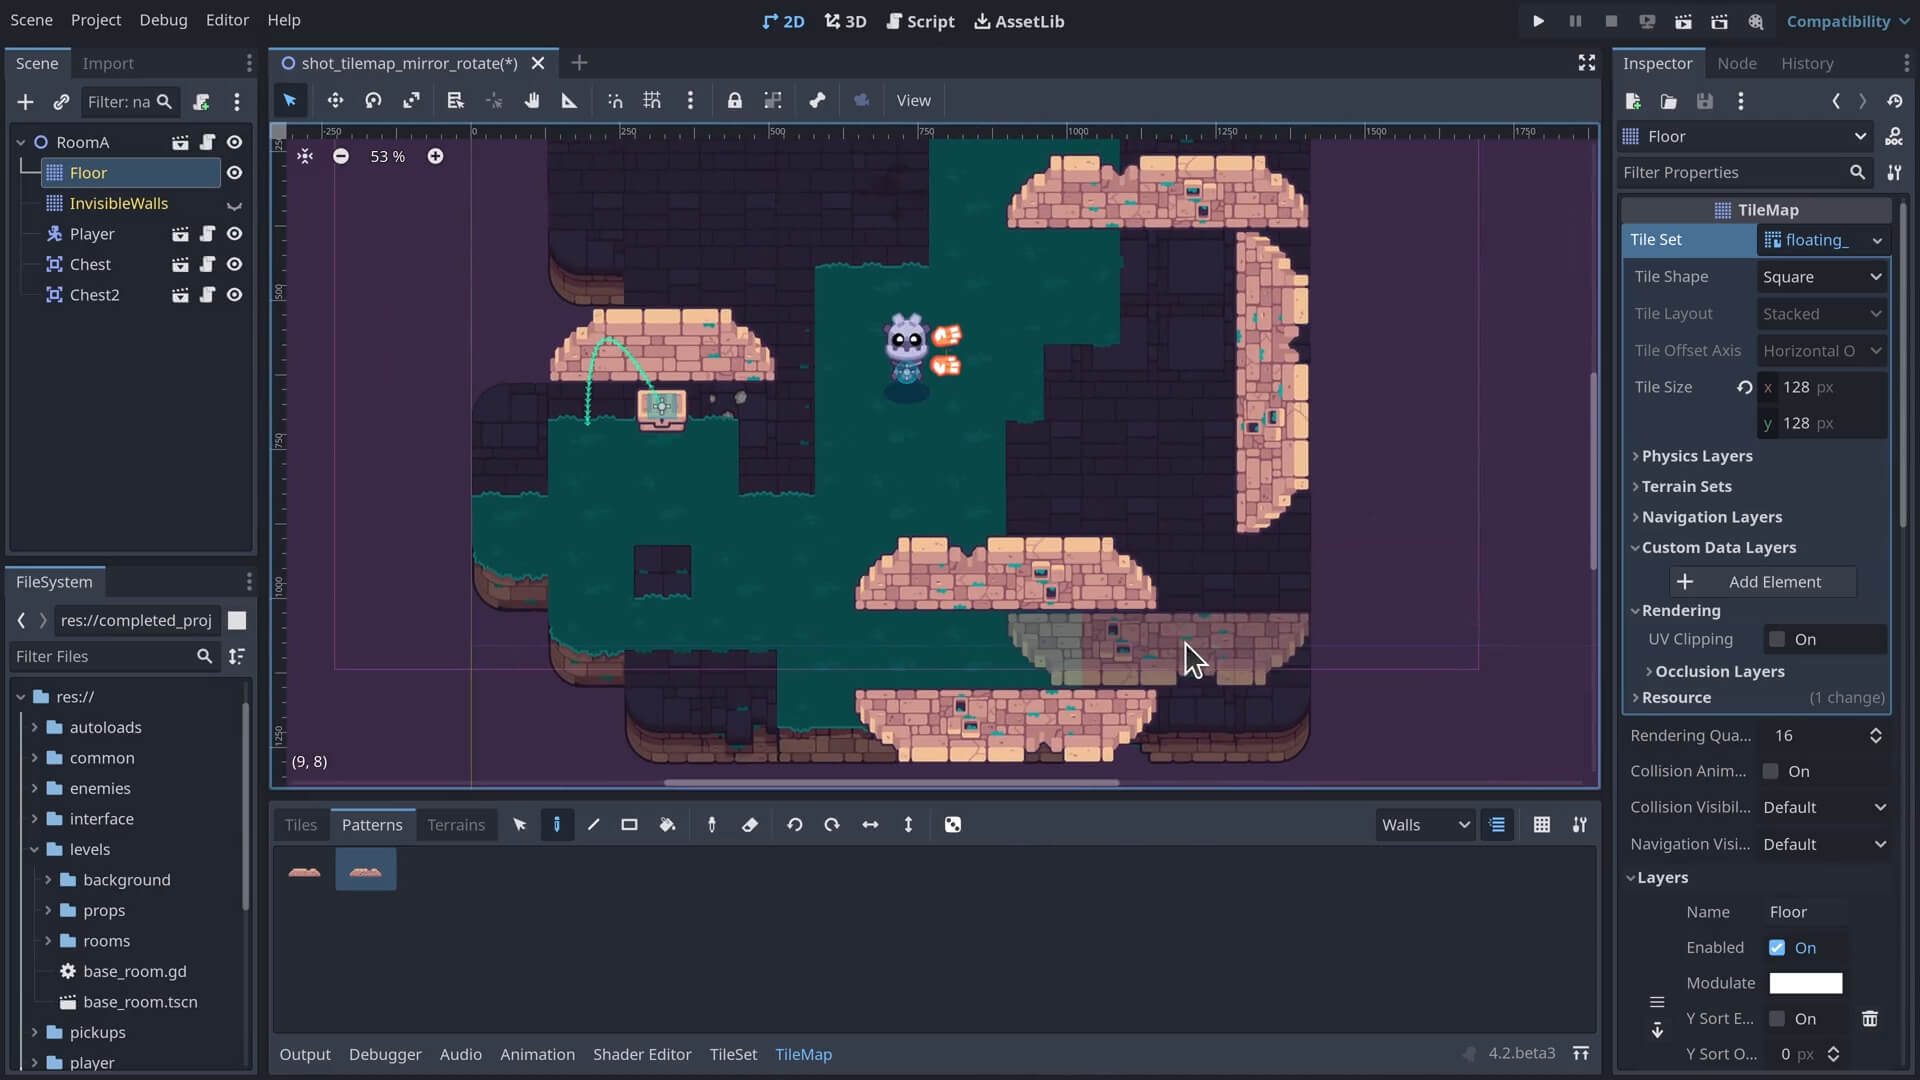
\includegraphics[scale = 0.2]{images/Godot_engine.jpg}
\caption{A Godot játékmotor visual scripting rendszere \cite{godot}}
\label{fig:godotengine}
\end{figure}

A Godot nagy és aktív közösséggel rendelkezik, amely rengeteg forrást, oktatóanyagot és fórumot biztosít a tanuláshoz és problémamegoldáshoz. A Godot felhasználóbarátnak számít, különösen a kezdők számára, köszönhetően a könnyű kialakításának, a különböző hardvereken nyújtott hatékony teljesítményének és az aktív közösségnek, amely folyamatosan hozzájárul a fejlesztéséhez. \cite{godot}

\SubSection{A Unity játékmotor}

A Unity egy nagy teljesítményű és sokoldalú játékmotor, amely támogatja a 3D-s és 2D-s játékok, valamint az interaktív szimulációk létrehozását. A 2005-ös megjelenése óta a Unity több fejlesztő számára elérhetőbbé tette a játékfejlesztést különböző platformokon. Dacára annak, hogy a Unity egy Mac OS X játékmotorként indult, mára már számos asztali, mobil, konzolos és virtuális valóság platformot támogat. Különösen népszerű az iOS és Android mobiljátékok fejlesztésében, a kezdő játékfejlesztők számára könnyen kezelhetőnek számít, és népszerű az indie játékfejlesztők körében.

A Unity lehetővé teszi a felhasználók számára, hogy 2D-s és 3D-s játékokat és játékélményeket hozzanak létre. A Unity elsődleges programozási nyelvének a C\# nyelv lett kiválasztva, hozzáférhetősége és sokoldalúsága miatt. A programozási tapasztalattól függetlenül a C\# felhasználóbarát környezetet biztosít a játékfejlesztésbe kezdő emberek számára. Egyszerű szintaxisa és az egyszerű felépítése zökkenőmentessé és élvezetessé teszi a tanulást és a kódírást. A C\# egy objektumorientált programozási (OOP) nyelv, amely tökéletesen illeszkedik a játékfejlesztéshez. \cite{unity2}

Aki nem ért annyira a programozáshoz, annak sem kell csüggednie, hiszen a Unity-nek is van egy beépített visual scripting rendszere, amely a Bolt névre hallgat. Ez egy kódolás nélküli megoldás, amely lehetővé teszi, hogy bárki létrehozzon AI-rendszereket és játéklogikát egy csomópontokon alapuló vizuális felület segítségével. A visual scripting mechanikával vizuálisan meg tudjuk tervezni és össze tudjuk kapcsolni a csomópontokat, hogy komplex interakciókat és viselkedéseket hozzunk létre anélkül, hogy egyetlen sor kódot kellene írnunk. Lehetővé teszi a nem fejlesztők számára, hogy részt vegyenek a játékfejlesztésben, mivel felhasználóbarát és intuitív módot kínál ötleteik életre keltéséhez. \cite{unity2} A Unity visual scripting rendszere \aref{fig:unityvisualscripting}. ábrán látható.

\begin{figure}[ht]
\centering
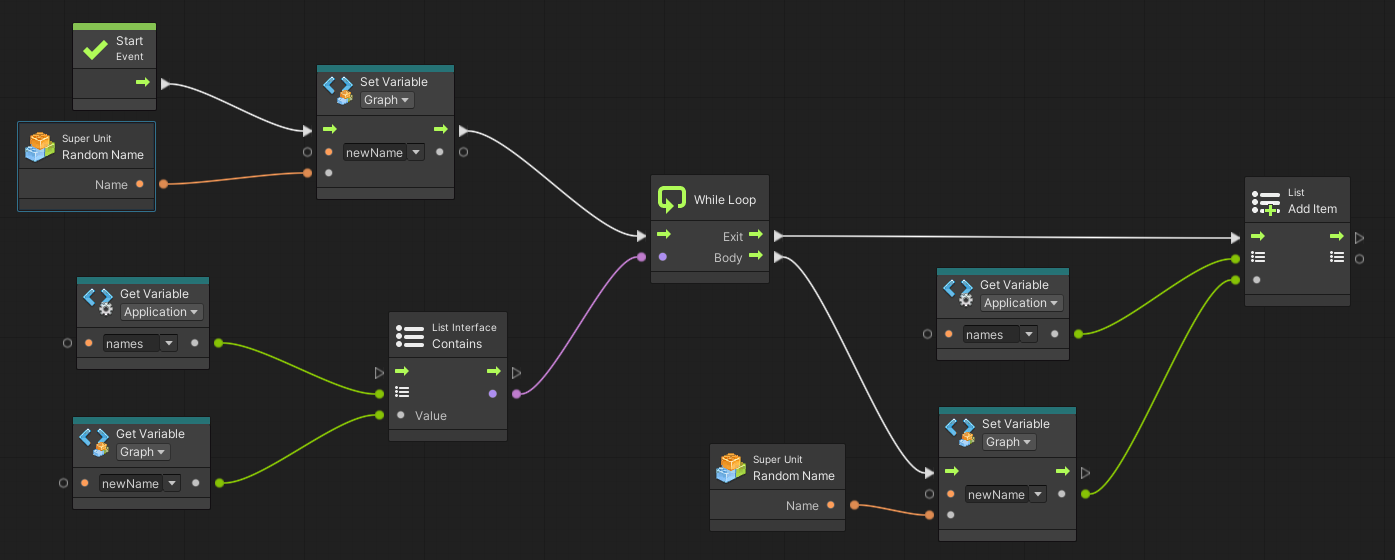
\includegraphics[scale = 0.3]{images/visual_scripting_unity.png}
\caption{A Unity Bolt névre hallgató visual scripting rendszere \cite{unity1}}
\label{fig:unityvisualscripting}
\end{figure}

Érdemes megjegyezni, hogy a visual scripting nem korlátozódik a játéklogikára. A Unity a shaderekhez és vizuális effektekhez is kínál vizuális szkriptelési megoldást Unity Shadergraph néven. A Shadergraph lehetővé teszi lenyűgöző vizuális effektek létrehozását az árnyékolók és effektek megtervezésével egy csomópont-alapú felületen keresztül. \cite{unity2}

A Unity Asset Store egy kincsesbánya, amely kiegészíti a Unity beépített funkcióit, és lehetővé teszi, hogy könnyedén fejleszthessük a játékunkat. Az ingyenes és fizetős assetek hatalmas választékával az Asset Store több mint 80 000 assethez biztosít hozzáférést, köztük 8000 ingyenes erőforráshoz, amelyeket megvásárlásukat követően közvetlenül a szerkesztőből importálhatunk a projektünkbe. Az Asset Store az assetek széles választékát kínálja az igényeinknek megfelelően. A kész modellektől, animációktól és textúráktól kezdve a sablonokon át a vizuális effektekig (VFX) minden megtalálható, ami ahhoz szükséges, hogy játékunkat szinesítsük, valamint értékes fejlesztési időt takarítsunk meg. \cite{unity2} A Unity Asset Store-jának egy kis részletettttttttttttttttttttttttttttttttt \aref{fig:unityassetstore}. ábrán megtekinthető.

\begin{figure}[ht]
\centering
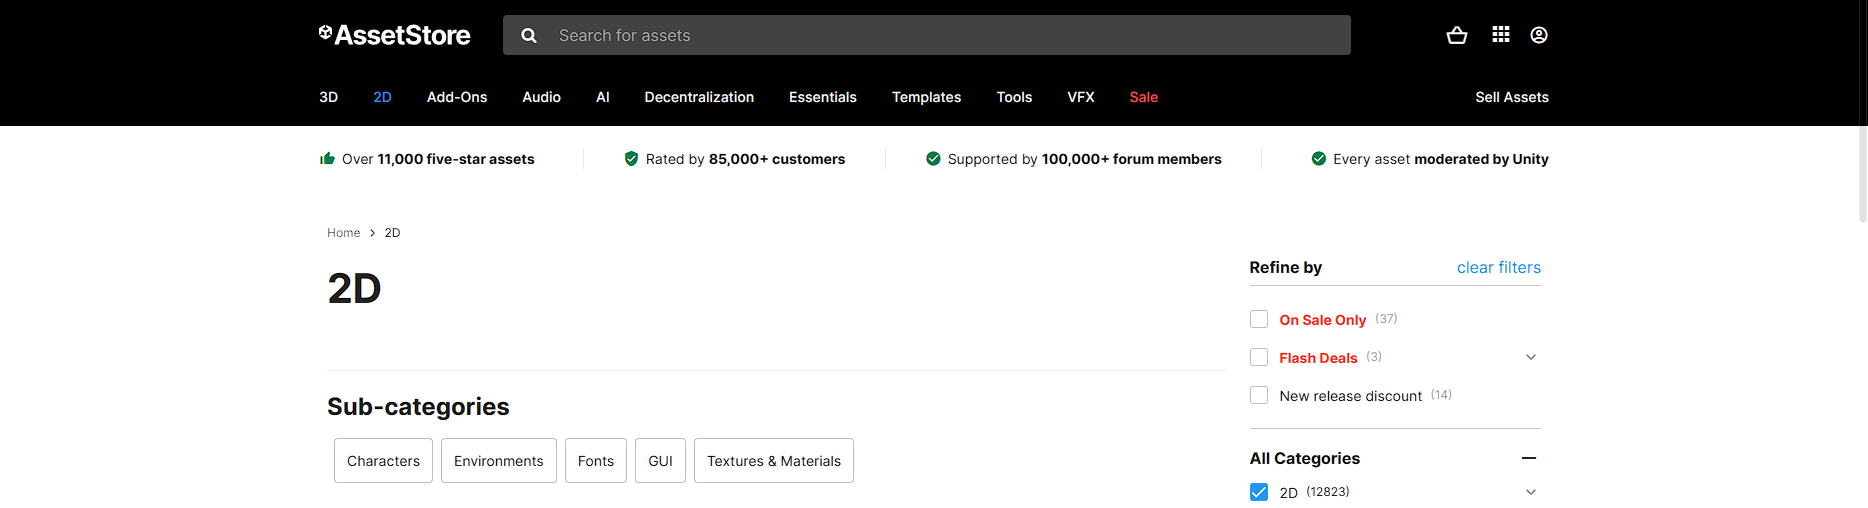
\includegraphics[scale = 0.3]{images/unity_asset_store.png}
\caption{A Unity Asset Store nevezetű boltja, ahonnan a játékunkhoz szerezhetjük be a megfelelő sprite-okat \cite{unityassetstore}}
\label{fig:unityassetstore}
\end{figure}

Unity egy virágzó közösséggel büszkélkedhet, amely felbecsülhetetlen erőforrásként szolgál a fejlesztők számára. A különböző platformok és fórumok segítségével csatlakozhatunk a hasonlóan gondolkodó emberekhez, támogatást kérhetünk, és közösen dolgozhatunk a többi emberrel a játékunk fejlesztése során. A Unity hivatalos fóruma egy nyüzsgő központot biztosít a fejlesztők számára, ahol vitatkozhatnak, kérdéseket tehetnek fel és megoszthatják tudásukat. Ez az információk kincsesbányája, ahol megoldásokat találhatunk a közös kihívásokra, új technikákat fedezhetünk fel, és naprakészek maradhatunk a legújabb iparági trendekkel kapcsolatban. A Reddit egy másik élénk közösség, ahol a Unity-rajongók összegyűlnek, hogy ötleteket cseréljenek, bemutassák munkájukat és támogassák egymást. Ezek a közösségek értékes platformként szolgálnak a világszerte működő fejlesztőkkel való kapcsolatteremtéshez, inspirációszerzéshez és tapasztalatcseréhez.  \cite{unity2}

Összességében a Unity nagyon jó választás a játékfejlesztéshez, mivel sokoldalú programozási nyelvet, bőséges tanulási forrásokat és egy élénk közösséget kínál.
